\documentclass[a4paper,11pt,cours]{nsi} 
\geometry{margin=2cm}



\setcounter{chapter}{1} % 1 de moins que le num de chapitre
%\creativecommonsfooter  %Pour marquer le doc
\begin{document}


\chapter{Second degré}
\section{Plusieurs formes pour un même polynôme}
\subsection{Fonction polynôme, forme développée}
\begin{definition}
	On appelle \textbf{fonction polynôme du second degré} toute fonction $f$ définie sur $\R$ telle qu'on puisse écrire pour tout $x\in\R$ :
	{\boldmath $$f(x)=ax^2+bx+c$$ }
	où $a$, $b$, et $c$ sont trois réels et $a\neq 0$.\\
	Cette écriture s'appelle la \textbf{forme développée} de $f$.
\end{definition}
\begin{itemize}
	\item 	$a\neq 0$, sinon $f$ serait une fonction affine.
	\item 	On dit aussi que $f$ est un \textbf{trinôme} du second degré.
\end{itemize}
\begin{exemple}[s]
	\begin{itemize}
		\item 	$f$ définie sur $\R$ par $\quad f(x)=3x^2-7x+2 \quad $ est une fonction polynôme du second degré :\\
		$\mathcal{D}_f=\R$, $\quad a=3$, $\quad b=-7 \quad$ et $\quad c=2$.
		\item 	$g$ définie sur $\R$ par $\quad x\mapsto -7x^2+11x-5 \quad$ aussi :	$\quad \mathcal{D}_g=\R$, $\quad a=-7$, $\quad b=11 \quad$ et $\quad c=-5$.
		\item 	$h$ définie sur $\R$ par $\quad h(x)=x^2+1 \quad$ également : $\quad \mathcal{D}_h=\R$, $\quad a=1$, $\quad b=0 \quad$ et $\quad c=1$.
		\item 	$k$ définie sur $\R$ par $\quad k(x)=x^3-(x+1)(x+2)(x+3)\quad$ est une fonction polynôme du second degré.
		En effet, pour tout $x\in\R$,
		\begin{tabbing}
			$k(x)$	\=	$=x^3-(x+1)(x+2)(x+3)$\\
			\>	$=x^3-(x^2+2x+x+2)(x+3)$\\
			\>	$=x^3-(x^2+3x+2)(x+3)$\\
			\>	$=x^3-[x^3+3x^2+2x+3x^2+9x+6]$\\
			\>	$=x^3-[x^3+6x^2+11x+6]$\\
			\>	$=x^3-x^3-6x^2-11x-6$\\
			\>	$=-6x^2-11x-6$
		\end{tabbing}
	\end{itemize}
\end{exemple}
\subsection{Forme factorisée}
\begin{definition}
	Soit $f$ une fonction polynôme de degré 2, définie pour tout $x\in\R$ par
	$$f(x)=ax^2+bx+c\qquad\qquad(a\neq 0)$$
	On dit que $f$ peut s'écrire sous \textbf{forme factorisée} s'il est possible d'écrire, pour tout $x\in\R$:
	\textbf{\boldmath $$f(x)=a(x-x_0)(x-x_1)$$}
	où $x_0$ et $x_1$ sont deux réels, éventuellement égaux.\\
\end{definition}

\begin{propriete}
	\textbf{Cette forme n'existe pas toujours : il existe des fonctions polynôme de degré 2 qui n'admettent pas de forme factorisée.}
\end{propriete}

\begin{demonstration}
	\carreauxseyes{16}{11.2}
\end{demonstration}

\begin{exemple}[s]
	\begin{itemize}
		\item 	$u$ définie sur $\R$ par $\quad u(x)=3x^2-9x+6\quad $ a pour forme factorisée :\\$u(x)=3(x-1)(x-2)$.\\
		En effet, pour tout $x\in\R$,
		\begin{tabbing}
			$3(x-1)(x-2)$	\=	$=3(x^2-2x-x+2)$\\
			\>	$=3(x^2-3x+2)$\\
			\>	$=3x^2-9x+6$
		\end{tabbing}
		\item 	$f$ définie sur $\R$ par $\quad f(x)=x^2 \quad$ est écrite sous forme factorisée :\\ pour tout $x\in\R$, $\quad f(x)=(x-0)(x-0)$.
		\item 	$g$ définie sur $\R$ par $\quad g(x)=x^2+1\quad$ n'admet pas de forme factorisée : en effet pour tout $x\in\R$, $\quad g(x)\geqslant1 \quad$ donc $g$
		ne s'annule pas sur $\R$.
	\end{itemize}
\end{exemple}

\subsection{Forme canonique}
\begin{definition}
	Soit $f$ une fonction polynôme de degré 2, définie pour tout $x\in\R$ par
	$$f(x)=ax^2+bx+c\qquad\qquad(a\neq 0)$$
	La \textbf{forme canonique} de $f$ est l'écriture suivante pour tout $x\in\R$ :
	{\boldmath $$f(x)=a(x-\alpha)^2+\beta$$}
	où $\alpha$ et $\beta$ sont deux réels.\\
\end{definition}

\begin{exemple}[s]
	\begin{enumerate}[label=\textbullet]

		\item 	$u$ définie sur $\R$ par $\quad u(x)=x^2+1\quad$ est écrite sous forme canonique.\\
		En effet, pour tout $x\in\R$, $$u(x)=1\times(x-0)^2+1$$
		\item 	$v$ définie sur $\R$ par $\quad v(x)=2x^2+4x-7 \quad$ a pour forme canonique\\ $v(x)=2(x+1)^2-9$.\\
		En effet, pour tout $x\in\R$,
		\begin{tabbing}
			$2(x+1)^2-9$	\=	$=2(x^2+2x+1^2)-9$\\
			\>	$=2x^2+4x+2-9$\\
			\>	$=2x^2+4x-7$\\
			\>	$=v(x)$
		\end{tabbing}
	\end{enumerate}
\end{exemple}

\begin{propriete}
	\textbf{Tout polynôme de degré 2 s'écrit de manière unique sous forme canonique :}
	{\boldmath $$f(x)=a(x-\alpha)^2+\beta$$}
\end{propriete}	

\begin{demonstration}
	\carreauxseyes{16}{16}
\end{demonstration}


\begin{encadrecolore}{consequence}{UGLiDarkBlue}
	Soit $f$ une fonction polynôme de degré 2, définie pour tout $x\in\R$ par
	$$f(x)=ax^2+bx+c\qquad\qquad(a\neq 0)$$
	En écrivant la forme canonique de $f$ : pour tout $x\in\R$,
	$$f(x)=a(x-\alpha)^2+\beta$$
	On a {\boldmath $$\alpha=-\dfrac{b}{2a}$$ et en posant $\Delta=b^2-4ac$ on a $$\beta=-\dfrac{\Delta}{4a}$$
		et par ailleurs $$\beta = f(\alpha)$$}
\end{encadrecolore}

\begin{demonstration}
	\carreauxseyes{16}{8}
\end{demonstration}

\begin{definition}
	Le réel $\quad \Delta=b^2-4ac \quad$ est appelé le \textbf{discriminant} de la fonction $f$.\\
	Nous verrons plus tard que \textbf{le signe de $\Delta$} est d'une grande importance pour résoudre des équations du second degré.
\end{definition}	
\subsection{Bilan}
\begin{center}\footnotesize
	\begin{tabular}{|c|c|c|}
		\hline
		\textbf{Nom} & \textbf{Expression} &\textbf{Commentaires} \\
		\hline
		&&\\
		forme développée & $f(x)=ax^2+bx+c$ & Existe toujours.\\
		&&On aboutit à cette forme en développant les deux autres. \\
		\hline
		&&\\
		forme factorisée & $f(x)=a(x-x_0)(x-x_1)$ & N'existe pas si $f$ ne s'annule pas dans $\R$. \\
		&&\\
		\hline
		&&\\
		forme canonique & $f(x)=a(x-\alpha)^2+\beta$ & Existe toujours. \\
		&&\\
		\hline
	\end{tabular}
\end{center}	


\section{Intérêts des deux premières formes}
\subsection{Intérêt de la forme développée}\ \\[-2em]
On peut l'utiliser pour vérifier que deux fonctions sont égales, en développant une des deux (ou les deux) et en comparant les formes 
développées.

\begin{exemple}
	Montrer que $k$ et $l$ définies sur $\R$ par $\quad k(x)=5(x+2)(x-4)\quad$ et $\quad l(x)=5(x-1)^2-45\quad$ sont la même fonction.\\[1em]
	\textbf{Méthode:}\\
	Pour tout $x\in\R$ :
	\begin{multicols}{2}
		d'une part,
		\begin{tabbing}
			$k(x)$	\= 	$=5(x+2)(x-4)$	\\
			\>	$=5[x^2-4x+2x-8]$	\\
			\>	$=5[x^2-2x-8]$\\
			\>	$=5x^2-10x-40$
		\end{tabbing}
		%\columnbreak
		d'autre part,
		\begin{tabbing}
			$l(x)$	\= 	$=5(x-1)^2-45$	\\
			\>	$=5(x^2-2x+1)-45$	\\
			\>	$=5x^2-10x+5-45$\\
			\>	$=5x^2-10x-40$
		\end{tabbing}
	\end{multicols}
	Donc pour tout $x\in\R$, $k(x)=l(x)$, les deux fonctions sont donc égales.
\end{exemple}
\subsection{Intérêt de la forme factorisée}
La forme factorisée est très utile pour \textbf{\boldmath résoudre l'équation $f(x)=0$, ou une inéquation du type $f(x)>0$.}

\begin{exemple}[\ 1]
	$f$ est définie sur $\R$ par $f(x)=-7(x-2)(x+4)$.\\
	{\boldmath Résoudre $f(x)=0$}
	\begin{tabbing}
		$f(x)=0$	\= 	$\quad\Leftrightarrow\quad -7(x-2)(x+4)=0$	\\
		\>	$\quad\Leftrightarrow\quad (x-2)(x+4)=0\qquad$ c'est une équation produit nul.\\
		\>	$\quad\Leftrightarrow\quad x-2=0\qquad$ \= 	ou $\qquad x+4=0$	\\
		\>	$\quad\Leftrightarrow\quad x=2\qquad$ \> 	ou $\qquad x=-4$
	\end{tabbing}
	0 admet 2 et -4 pour antécédents par $f$.
\end{exemple}

\begin{exemple}[\ 2]
	{\boldmath Résoudre $f(x)>0$}\\
	Avec un tableau de signes :
	\begin{center}
		\begin{tikzpicture}
			\tkzTabInit[color,lgt=3.5,espcl=2]	{$x$ /1,$x-2$ /1,$x+4$ /1,$(x-2)(x+4)$ /1,$-7(x-2)(x+4)$ /1}
			{$-\infty$,$-4$,$2$,$+\infty$}
			\tkzTabLine{,-,t,-,z,+,}
			\tkzTabLine{,-,z,+,t,+,}
			\tkzTabLine{,+,z,-,z,+,}
			\tkzTabLine{,-,z,+,z,-,}
		\end{tikzpicture}\\
		
		$$\mathcal{S}=\oio{-4}{2}$$
	\end{center}
\end{exemple}
\section{Intérêts de la forme canonique}

C'est la forme la plus intéressante. Elle permet de :
\begin{itemize}
	\item 	Donner le tableau de variation de la fonction.
	\item 	Tracer la courbe représentative de la fonction rapidement.
	\item 	Résoudre les équations du type $f(x)=k$  ou les inéquations du type $f(x)>k$.
\end{itemize}
\subsection{Deux propriétés}
\begin{propriete}[\ 1]
	Soit $f$ une fonction polynôme de degré 2 sous forme canonique :\\ pour tout $x\in\R$, $f(x)=a(x-\alpha)^2+\beta$.\\
	\begin{itemize}
		\item 	\textbf{Si {\boldmath $a>0$}} alors on a :\\
		\begin{center}
			\begin{tikzpicture}
				\tkzTabInit[color]{$x$/1,$f$/2}{$-\infty$,$\alpha$,$+\infty$}
				\tkzTabVar{+/,-/$\beta$,+/}
			\end{tikzpicture}
		\end{center}
		\item 	\textbf{Si {\boldmath $a<0$}} alors on a :\\
		\begin{center}
			\begin{tikzpicture}
				\tkzTabInit[color]{$x$/1,$f$/2}{$-\infty$,$\alpha$,$+\infty$}
				\tkzTabVar{-/,+/$\beta$,-/}
			\end{tikzpicture}
		\end{center}
	\end{itemize}	
\end{propriete}

\newpage

\begin{demonstration}
	\textbf{\boldmath Si $a>0$: }\\
	On décompose la fonction :
	\begin{center}
		\begin{tikzpicture}
			\tkzTabInit[color,lgt=3.5]{$x$/1,Variations de $x\mapsto x-\alpha$ /2,Variations de $x\mapsto (x-\alpha)^2$ /2,Variations de $x\mapsto a(x-\alpha)^2$ /2, Variations de $x\mapsto 
			a(x-\alpha)^2+\beta$/2}{$-\infty$,$\alpha$,$+\infty$}
			\tkzTabVar{-/, R / /,+/}
			\tkzTabVal{1}{3}{0.5}{$\alpha$}{0}
			\tkzTabVar{+/,-/0,+/}
			\tkzTabVar{+/,-/0,+/}		
			\tkzTabVar{+/,-/$\beta$,+/}	
		\end{tikzpicture}
	
	
	\end{center}
	\textbf{\boldmath Si $a<0$: } On procède de la même manière.		\end{demonstration}

\begin{propriete}[\ 2]
	Avec les notations précédentes,
	
	\begin{itemize}
		\item 	$\mathcal{C}_f$, la courbe représentative de $f$ dans un repère orthogonal, est \textbf{une parabole de sommet}
		{\boldmath $\pc{S}{\alpha}{\beta}$}.\\
		Elle admet pour \textbf{axe de symétrie} la droite d'équation {\boldmath $x=\alpha$}.
		\item 	\textbf{Si {\boldmath $a>0$} alors}
		\begin{itemize}
			\item 	$f$ admet un \textbf{minimum} pour $x=\alpha$, celui-ci vaut $f(\alpha)$, c'est-à-dire $\beta$.
			\item 	On dit que $\mathcal{C}_f$ est « tournée vers le haut ».
		\end{itemize}
		\item 	\textbf{Si {\boldmath $a<0$} alors}
		\begin{itemize}
			\item 	$f$ admet un \textbf{maximum} pour $x=\alpha$, celui-ci vaut $f(\alpha)$, c'est-à-dire $\beta$.
			\item 	On dit que $\mathcal{C}_f$ est « tournée vers le bas » .\\
		\end{itemize}
	\end{itemize}
\end{propriete}

\subsection{Tracer la courbe représentative d'une fonction polynôme du second degré}
\begin{exemple}[\ 1]
	Soit $h$ la fonction définie sur $\R$ par $\quad h(x)=\dfrac{1}{2}(x-3)^2-2$.\\
	Soit $\repaff$ un repère orthonormé du plan.
	\begin{multicols}{2}
		\begin{itemize}
			\item 	$a=\dfrac{1}{2}$, $\quad \alpha=3$, $\quad \beta=-2$.
			\item 	$h$ est strictement décroissante sur $\iif{3}$ et strictement croissante sur $\fii{3}$.
			\item 	$h$ présente un minimum pour $x=3$, il vaut $-2$.
			\item 	$\mathcal{C}_h$ est une parabole « tournée vers le haut », de sommet $\pc{S}{3}{-2}$ et d'axe de symétrie $x=3$.
			\item 	Pour compléter le tracé de la courbe, on calcule par exemple $h(5)=0$ et $h(6)=2,5$ et on complète par symétrie.
		\end{itemize}
		
		\columnbreak
		
		\begin{center}
			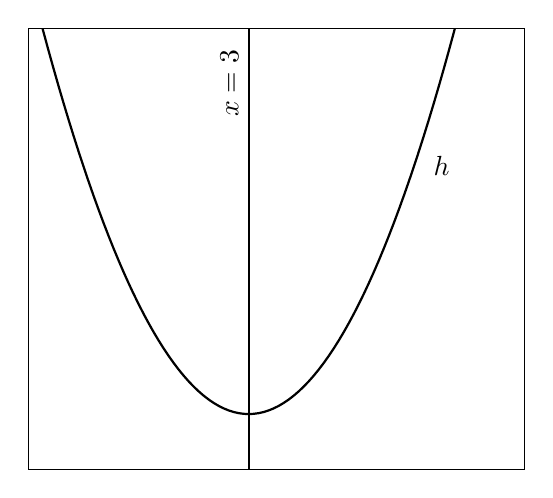
\begin{tikzpicture}[scale=.7]
				\draw[fill=white] (-1,-3) rectangle (8,5);
				\repereal{-1}{-3}{8}{5}
				\clip (-1,-3) rectangle (8,5);
				\def\F{.5*(\x-3)*(\x-3)-2}
				\draw [thick, domain = -1:8, samples = 100] plot( \x,{\F});
				\draw [thick](3,-3)  -- (3,4)node[above,rotate=90]{$x=3$} -- (3,5);
				\pointc{3}{-2}{3}{-2}{S}
				\point{5}{0}{}
				\point{6}{2.5}{}
				\draw (6.5,2.5)node{$\courbe{h}$};
			\end{tikzpicture}
		\end{center}
	\end{multicols}
	\ \\[-2em]
\end{exemple}

\begin{exemple}[\ 2]
	Soit $p$ la fonction définie sur $\R$ par $\quad p(x)=-(x+2)^2+5$.\\
	Soit $\repaff$ un repère \textbf{orthogonal} du plan.
	\begin{multicols}{2}
		\begin{itemize}
			\item 	$a=-1$, $\quad \alpha=-2$, $\quad \beta=5$.
			\item 	$p$ est strictement croissante sur $\iif{-2}$ et strictement décroissante sur $\fii{-2}$.
			\item 	$p$ présente un maximum pour $x=-2$, il vaut $5$.
			\item 	$\mathcal{C}_p$ est une parabole « tournée vers le bas », de sommet $\pc{S}{-2}{5}$ et d'axe de symétrie $x=-2$.
			\item 	Pour compléter le tracé de la courbe, on calcule par exemple $p(-3)=4$ et $p(-4)=1$ et on complète par symétrie.
		\end{itemize}
		
		\columnbreak
		
		\begin{center}
			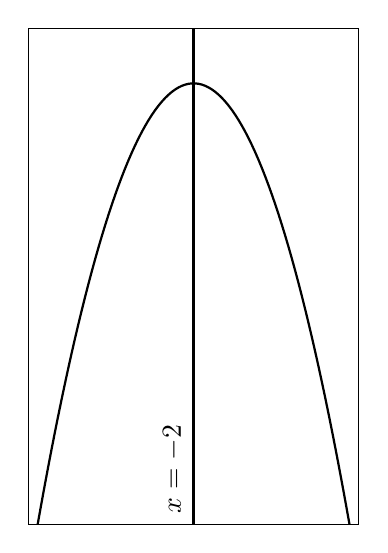
\begin{tikzpicture}[scale=.7]
				\draw[fill=white] (-5,-3) rectangle (1,6);
				\repereal{-5}{-3}{1}{6}
				\clip (-5,-3) rectangle (1,6);
				\def\F{-(\x+2)*(\x+2)+5}
				\draw [thick, domain = -5:1, samples = 100] plot( \x,{\F});
				\draw [thick](-2,-3)  -- (-2,-2)node[above,rotate=90]{$x=-2$} -- (-2,6);
				\pointc{-2}{5}{-2}{5}{S}
				\draw (6.5,2.5)node{$\courbe{h}$};
				\point{-3}{4}{}
				\point{-4}{1}{}
			\end{tikzpicture}
		\end{center}
	\end{multicols}
	\ \\[-2em]
\end{exemple}
\subsection{Résolutions d'équations et d'inéquations  avec la forme canonique}

Il est bon de savoir appliquer les méthodes des exemples suivants mais nous allons voir une méthode plus pratique au \textbf{IV}.\\
\begin{exemple}[\ 1]
	Reprenons la fonction du deuxième exemple et résolvons $p(x)=1$ :
	\begin{tabbing}
		$p(x)=1$	\= 	$\quad\Leftrightarrow\quad -(x+2)^2+5=4$	\\
		\>	$\quad\Leftrightarrow\quad -(x+2)^2=-1$	\\
		\>	$\quad\Leftrightarrow\quad (x+2)^2=1$	\\
		\>	$\quad\Leftrightarrow\quad x+2=1\qquad$ \= ou	$\qquad x+2=-1$ \\
		\>	$\quad\Leftrightarrow\quad x=-1\qquad$ \> ou	$\qquad x=-3$ 
	\end{tabbing}
	$\mathcal{S}=\left\lbrace\ -1\ ;\ -3\ \right\rbrace$.\\
	
\end{exemple}

\begin{exemple}[\ 2]
	Reprenons la fonction du premier exemple et résolvons $h(x)>3$ :
	\begin{tabbing}
		$h(x)>3$	\= 	$\quad\Leftrightarrow\quad \dfrac{1}{2}(x-3)^2-2>3$	\\[0.5em]
		\>	$\quad\Leftrightarrow\quad \dfrac{1}{2}(x-3)^2>5$	\\[0.5em]
		\>	$\quad\Leftrightarrow\quad (x-3)^2>10$	\\
		\>	$\quad\Leftrightarrow\quad x-3<-\sqrt{10}\qquad$ \= ou	$\qquad x-3>\sqrt{10}$ \\
		\>	$\quad\Leftrightarrow\quad x<3-\sqrt{10}\qquad$ \> ou	$\qquad x>3+\sqrt{10}$ \\
	\end{tabbing}
	$\mathcal{S}=\iio{3-\sqrt{10}}\cup\oii{3+\sqrt{10}}$.\\
\end{exemple}


\section{Utilisation du discriminant}
\subsection{Pour déterminer la forme factorisée si elle existe}
\begin{propriete}
	Soit $f$ une fonction polynôme de degré 2, définie pour tout $x\in\R$ par
	$$f(x)=ax^2+bx+c\qquad\qquad(a\neq 0)$$
	En écrivant la forme canonique de $f$, pour tout $x\in\R$ on a
	$$f(x)=a\left(x+\dfrac{b}{2a}\right)^2-\dfrac{\Delta}{4a}$$
	avec, rappelons-le, $\Delta=b^2-4ac$.
	\begin{itemize}
		\item	Si $\Delta<0$ alors $f$ ne peut s'écrire sous forme factorisée.
		\item 	Si $\Delta=0$ alors on pose {\boldmath$x_0=-\dfrac{b}{2a}$}, la forme factorisée de $f$ est alors : pour tout $x\in\R$,
		{\boldmath$$f(x)=a(x-x_0)^2$$}
		\item 	Si $\Delta>0$ alors on pose {\boldmath $x_1=\dfrac{-b-\sqrt{\Delta}}{2a}$ et $x_2=\dfrac{-b+\sqrt{\Delta}}{2a}$}, 
		la forme factorisée de $f$ est alors : pour tout $x\in\R$,
		{\boldmath $$f(x)=a(x-x_1)(x-x_2)$$}
	\end{itemize}
\end{propriete}
\begin{demonstration}
	\carreauxseyes{16}{18.4}
\end{demonstration}



\begin{exemple}[s]
	\begin{itemize}
		\item 	Soit $f$ définie sur $\R$ par $\quad f(x)=3x^2-9x+6$.\\
		On calcule le discriminant de $f$ :
		\begin{tabbing}
			$\Delta$	\=	$=(-9)^2-4\times 3\times 6$\\
			\>	$=81-72$\\
			\>	$=9$
		\end{tabbing}
		Ce discriminant est positif et $\sqrt{\Delta}=3$. Calculons $x_1$ et $x_2$ :\\
		
		$x_1=\dfrac{9-3}{2\times 3}\quad$ donc $\quad x_1=1\quad$ et $\quad x_2=\dfrac{9+3}{2\times 3} \quad$ donc $\quad x_1=2$.\\
		
		Par suite, la forme factorisée de $f$ est alors : pour tout $x\in\R$,
		{\boldmath $$f(x)=3(x-1)(x-2)$$}
		Ce qu'on peut vérifier en développant.
		
		\item 	Soit $f$ définie sur $\R$ par $f(x)=-4x^2+x-3$
		\begin{tabbing}
			$\Delta$	\=	$=1^2-4\times (-4)\times(-3)$\\
			\>	$=1-48$\\
			\>	$=-47$
		\end{tabbing}
		Ce discriminant étant négatif, $f$ n'admet pas de forme factorisée dans $\R$.
		
		\item 		Soit $f$ définie sur $\R$ par $\quad f(x)=4x^2+4x+1$.\\
		$\Delta=4^2-4\times 4\times1=16-16=0$.\\
		Ce discriminant est nul, on calcule 
		$x_0=\dfrac{-4}{2\times 4}$, c'est-à-dire $x_0=-\dfrac{1}{2}$ et la forme factorisée de $f$ est alors : 
		pour tout $x\in\R$,
		{\boldmath $f(x)=4\left(x+\dfrac{1}{2}\right)^2$}
	\end{itemize}
\end{exemple}

\subsection{Pour déterminer les solutions de $ax^2+bx+c=0$}


\begin{propriete}
	On considère l'équation 
	{\boldmath$$ax^2+bx+c=0\qquad\qquad(a\neq 0)$$}
	On appelle \textbf{discriminant de l'équation} le réel $\Delta=b^2-4ac$.
	\begin{itemize}
		\item	Si $\Delta<0$ alors l'équation \textbf{n'admet pas de solutions réelles}.
		\item 	Si $\Delta=0$ alors l'équation admet pour unique solution {\boldmath$x_0=-\dfrac{b}{2a}$}.
		\item 	Si $\Delta>0$ alors l'équation admet 2 solutions réelles : {\boldmath $$x_1=\dfrac{-b-\sqrt{\Delta}}{2a}\qquad\text{et}\qquad 
			x_2=\dfrac{-b+\sqrt{\Delta}}{2a}$$}
	\end{itemize}
\end{propriete}

\begin{demonstration}
	\carreauxseyes{16}{12}
\end{demonstration}
\begin{remarque}
	L'équation précédente s'écrit $$f(x)=0$$ 
	où $f$ est la fonction polynôme de degré 2, définie pour tout $x\in\R$ par
	$$f(x)=ax^2+bx+c\qquad\qquad(a\neq 0)$$
	Une solution éventuelle de l'équation $f(x)=0$ s'appelle \textbf{une racine} de $f$.
\end{remarque}

\begin{exemple}[ 1]
	On considère l'équation $\quad 5x^2-2x+1=0$.\\
	Son discriminant est $\Delta = (-2)^2-4\times 5\times1$, c'est à dire $-16$.\\
	Il est négatif, cette équation n'admet pas de solution réelle.
\end{exemple}


\begin{exemple}[ 2]
	On considère l'équation $\quad -9x^2+6x-1=0$.\\
	Son discriminant est $\Delta = 6^2-4\times (-9)\times(-1)$, c'est à dire $0$.\\
	Cette équation a donc pour solution $\dfrac{-6}{2\times 9}$, c'est à dire $-\dfrac{1}{3}$.
\end{exemple}

\begin{exemple}[ 3]
	On considère l'équation $\quad 2x^2-6x+4=0$.\\
	Son discriminant est $\Delta = (-6)^2-4\times 2\times 4$, c'est à dire $4$.\\
	Cette équation admet donc deux solutions :\\
	$x_1=\dfrac{6-\sqrt{4}}{2\times 2}$, c'est à dire $x_1=1$, \quad	et $x_2=\dfrac{6+\sqrt{4}}{2\times 2}$, c'est 
	à dire $x_2=2$.
\end{exemple}


\subsection{Pour déterminer le signe d'une expression du second degré}
\begin{propriete}
	Soit $f$ une fonction polynôme de degré 2, définie pour tout $x\in\R$ par
	$$f(x)=ax^2+bx+c\qquad\qquad(a\neq 0)$$
	\begin{itemize}
		\item	Si $\Delta<0$ alors \textbf{\boldmath pour tout $x\in\R$, $f(x)$ est du signe de $a$.}
		\item 	Si $\Delta=0$ alors en appelant $x_0$ l'unique racine de $f$, \textbf{\boldmath $f(x_0)=0$ et pour tout $x\neq x_0$, $f(x)$ est 
			du 
			signe de $a$}
		\item 	Si $\Delta>0$ alors en appelant $x_1$ la plus petite racine de $f$ et $x_2$ l'autre :
		\begin{itemize}
			\item 	\textbf{\boldmath pour tout $x\in\iio{x_1}\cup\oii{x_2}$, $f(x)$ est du signe de $a$.}
			\item 	{\boldmath $f(x_1)=f(x_2)=0$}
			\item 	\textbf{\boldmath pour tout $x\in\oio{x_1}{x_2}$, $f(x)$ est du signe opposé à celui de $a$.}
		\end{itemize}
	\end{itemize}
\end{propriete}	


\begin{demonstration}
	\carreauxseyes{16}{4.8}\\

	\carreauxseyes{16}{16}
\end{demonstration}	



\begin{exemple}
	Résoudre dans $\R$ l'inéquation $3x^2+x-14\leqslant 0$.\\
	
	\emph{Sans être explicite, on étudie le signe de la fonction $f$ définie sur $\R$ par $f(x)=3x^2+x-14$.}\\
	Le discriminant du trinôme est $1^2+4\times 3\times 14=169=13^2$, donc ce trinôme s'annule pour \\
	
	$x_1=\dfrac{-1-13}{2\times3}=-\dfrac{7}{3}$ 
	et pour $x_2=\dfrac{-1+13}{2\times3}=2$.\\
	
	$a$ est strictement positif car vaut 3. On en conclut que 
	\begin{itemize}
		\item 	\textbf{\boldmath pour tout $x\in\iio{x_1}\cup\oii{x_2}$, $3x^2+x-14>0$.}
		
		\item 	\textbf{\boldmath pour tout $x\in\fif{-\dfrac{7}{3}}{2}$, $3x^2+x-14\leqslant 0$.}
	\end{itemize}	
\end{exemple}


\end{document}
